$G$を非コンパクトな実線型半単純Lie群,$K$を$G$の極大コンパクト部分群で$G$のCartan対合$\Theta$に対して$K = \Theta K $なるものとする.$\ge = \ka \oplus \pe $を$\Theta$の微分$d\Theta$による$\ge$のCartan分解とするとき,$G/K$は$\pe$と$\pe \ni X\mapsto e^{X}K\in G/K $により微分同相である.

$H$を$G$の非コンパクトかつ連結成分有限個の閉部分群で,$H = \Theta H$を満たすものとし,$\ge$のKilling形式を$B$とする.$\per{\ha}\defeq \{W\in \ge\mid B(W, \ha) = \{0\} \} $とするとき,$G/K$と$\pe$の微分同相についてより強い次の構造定理が知られている.

\begin{thm*}(\cite[Lemma~6.1]{kob89})\label{thm:kob89-lem6.1}  
  $\pi\colon  (\ha\cap\pe)\oplus (\per{\ha}\cap \pe) \ni (Y, Z)\mapsto e^{Y}e^{Z}\cdot o_K \in G/K $は上への微分同相である.
\end{thm*}
この定理を用いて$X\in \pe$に対し,${(Y(X), Z(X))\defeq \inv{\pi}(e^X\cdot K)\in (\ha\cap\pe)\oplus (\per{\ha}\cap \pe)}$と定義する.

$G/K$に$\ge$のKilling形式$B$から定まるRiemann計量によってRiemann多様体の構造を定める.$G$の単位元の$G/K$での像$eK$を通る$G/K$の極大測地線は$B(X, X) = 1 $なる$X\in \pe$によって$e^{tX}K $,$t\in \real$と書ける.\Cref{thm:kob89-lem6.1}より任意の$t\in \real$に対して$e^{tX}K = e^{Y(tX)}e^{Z(tX)}K $である.

$G = \SU(1,1) $,$H = \SO(1,1) $とするとき,$t\in \real$に対し,$Y(tX) $は\Cref{fig:y-and-z}に図示するような幾何学的な意味を持つ.\Cref{fig:y-and-z}は{\Poincare}円板における測地線$e^{tX}K$ (赤色の斜め線) とその上の一点$e^{tX}K$から$eK$の$H$軌道 (中央の直線) に下ろした垂線の足 (緑の丸) が$e^{Y(tX)}K $である.
\begin{figure}[H]
  \centering
  %   \raggedleft
  %   \raggedrightp
  %   \includegraphics[scale=0.08]{graph/fig1.jpg}
  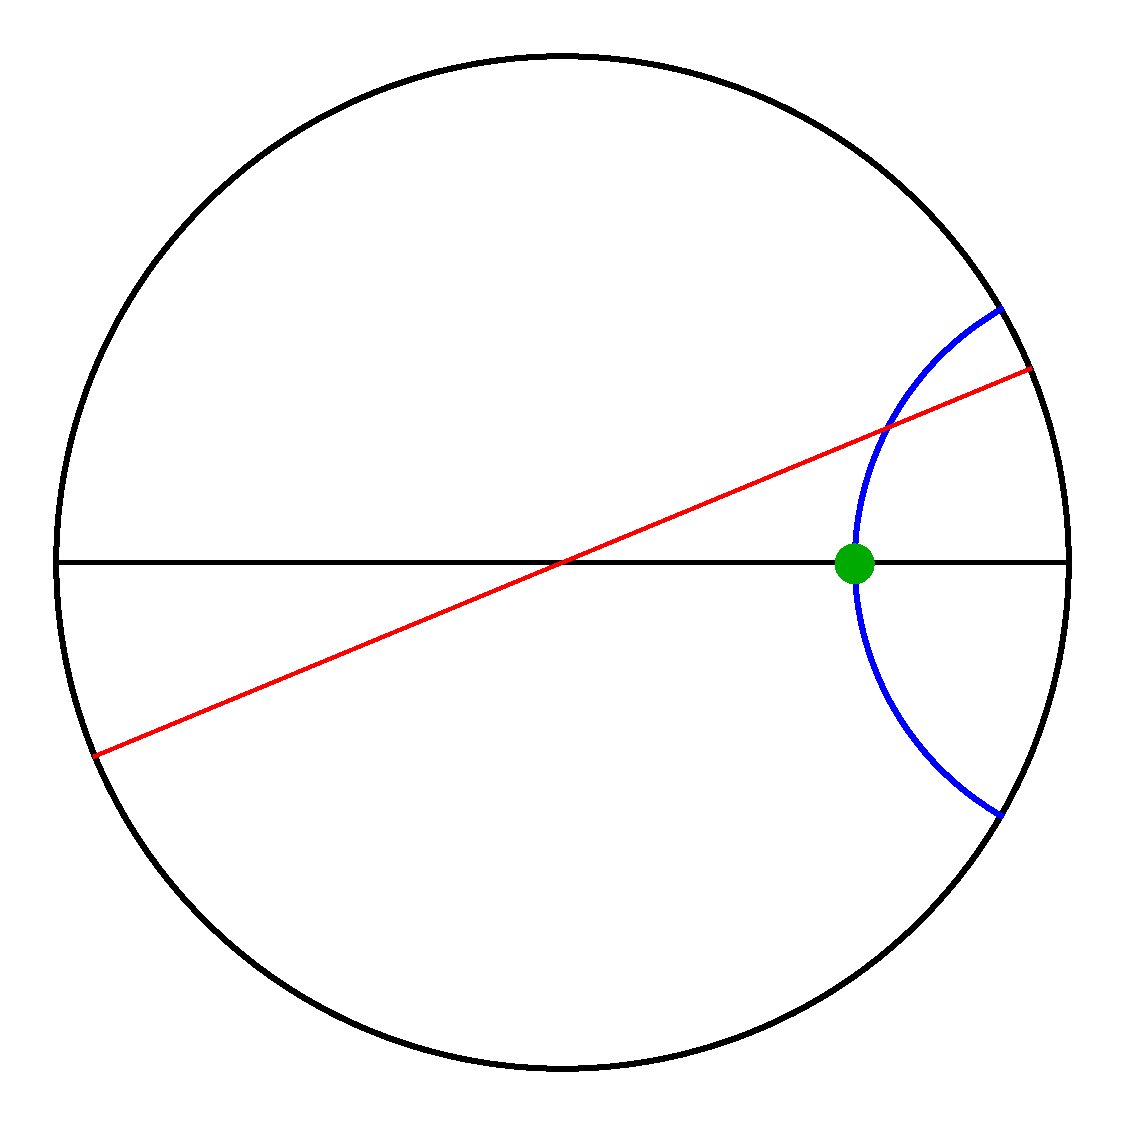
\includegraphics[scale=0.3]{../graph/y-and-z.pdf}
  \caption{{\Poincare}円板における$Y(tX) $の幾何学的意味}
  \label{fig:y-and-z}
\end{figure}

本論文では小林俊行氏による次の問題 (後述の\Cref{prob:1121}) について考察し,$G$が実階数1の実半単純Lie群の場合に肯定的な結果を得た.
\begin{prob*}(小林俊行氏による)
  $X\in  \pe$に対して,$Y(\real X)$が$ \ha\cap \pe$の有界な部分集合であることと次の条件は同値であるか?
  \begin{cond*}
    \leavevmode\vspace{-1em}
    \begin{itemize}
    \item $X\in \per{\ha}\cap\pe $
    \item[] もしくは
    \item $[X_1, X_2] \neq 0 $かつ$X\in \ge_{s}' $,
    \item[] もしくは
    \item $[X_1, X_2] \neq 0 $かつ$\pe\cap \ze(\ge') \nsubset \ha  $
    \end{itemize}
    である.
  \end{cond*}

  記号は次のとおりとする.
  \begin{itemize}
  \item $X = X_1 + X_2 $はベクトル空間としての分解$\pe =(\pe\cap \ha)\oplus(\pe\cap\per{\ha}) $に対応する$X\in \pe$の分解とする.
  \item $\ge ' $は$\ha$と$X$が生成する$\ge$の部分Lie環とする.$\ha = \theta \ha$より$\theta \ge' = \ge'$である.

    よって$\ge'_{s} \defeq [\ge',\ge'] $とすると$\ge' = \ze(\ge') \oplus \ge'_{s} $と分解される.
  \end{itemize}
\end{prob*}

ここで$G$が実階数1のとき,上の条件と$X\in \{0\}\cup\pe\setminus\ha $は同値である (後述する\Cref{lem:basic-prob}の3).



\Cref{prob:1121}の背景を説明するために\cite{ber88}の内容についてふれる.

まずいくつか用語を準備する.$G$を実簡約Lie群,$H$を$G$の閉部分群とし,$G/H$には左Haar測度$\mu_{G/H} $が存在すると仮定する.局所有界関数$r\colon G\to \real_{\geq 0} $がproperなradial functionであるとは,$r$が次の4条件を満たすことである.
\begin{enumerate}
\item $e\in G$を単位元とするとき$r(e) = 0 $である.
\item 任意の$g\in G$に対し$r(g) = r(\inv{g})\geq 0  $である.
\item 任意の$g_1,g_2\in G$に対し$r(g_1g_2)\leq r(g_1) + r(g_2)  $である.
\item 任意の$R\geq 0$に対し,$B(R)\defeq \{g\in G\mid r(g)\leq R \} $は$G$の相対コンパクト集合である.
\end{enumerate}
properなradial function $r\colon G\to \real_{\geq 0} $から$r_{G/H}(gH)\defeq \inf_{h\in H}\{r(gh) \}$により定まる${r_{G/H}\colon G/H\to \real_{\geq 0}}$を$G/H$上のradial functionという.

$G/H$にはstandard measureと呼ばれる,次を満たす非自明なBorel 測度$m_X $が存在する.単位元のコンパクトな近傍で$B = \inv{B} $なる任意の$B\subset G$と任意の$g\in B$,$x\in G/H$に対し,ある定数$C_B\geq 0 $が存在して$g\cdot m_X \leq C_B m_X$,$ \inv{C_B} < m_X(Bx) < C_{B}$である.

$d = \inf\{d'\geq 0\mid \text{ある } C > 0\text{が存在して }  m_X(B(r))\leq C(1+r)^{d'}\} $であるとき,$G/H$のランクは$d$であると言う.

$G$の既約ユニタリ表現$V$が$G$の正則表現$L^2(G/H)$の既約分解に出現する必要条件は,非自明な$G$-絡作用素$\alpha_V\colon (C_c(G/H))^{\infty}\to V $が存在し,任意の$v\in V^{\infty} $,$d' > d$に対して$\dint_{G/H}\lbig|\beta_V(v)(x)(1+r(x))^{-d/2} \rbig|^2\; dx < \infty $なることである.ただし$\beta_V $は次の命題により$\alpha_V $と対応する$G$-絡作用素$\beta_V\colon V^{\infty}\to C(G/H)^{\infty}  $とする.
\begin{prop*}(\cite[p.~678]{ber88})
  $G/H$の左Haar測度$\mu_{G/H} $を1つ固定する.次の同型写像が存在する.$\Hom_{G}((C_c(G/H))^{\infty}, V )\to \Hom_{G}(V^{\infty}, C(G/H)^{\infty}) $,$\alpha_V\mapsto \beta_V$ただし任意の$v\in V$,$\phi \in  (C_c(G/H))^{\infty} $に対し$ \lyama v,\alpha_V(\phi)\ryama_{V} = \dint_{G/H}\beta_V(v)\phi d\mu_X  $である.
\end{prop*}

% $G$を実簡約Lie群,$H$を$G$の閉部分群とし,ある可換部分群$B\subset G$が存在して$G = KBH $というCartan分解を持つとする.任意の$X\in \Lie B$に対して$Y(\real X) $が有界であれば,$G/H$がランク$d \defeq \dim B $となるための条件のうちの1つである,「ある定数$C > 0$が存在して,任意の$X\in \Lie B$に対し,$d_{G/K}(\exp(-X)\cdot o_K, o_K )  - \inf\{d_{G/K}(\exp(-X)\cdot o_K,h\cdot o_K ) \mid h\in H\}\leq C$であること」が満たされる.

以上が本修士論文の表現論的な背景である.
